% !TeX spellcheck = en_GB
% !TeX program = lualatex
%
% v 2.3  Feb 2019   Volker RW Schaa
%		# changes in the collaboration therefore updated file "jacow-collaboration.tex"
%		# all References with DOIs have their period/full stop before the DOI (after pp. or year)
%		# in the author/affiliation block all ZIP codes in square brackets removed as it was not %         understood as optional parameter and ZIP codes had bin put in brackets
%       # References to the current IPAC are changed to "IPAC'19, Melbourne, Australia"
%       # font for ‘url’ style changed to ‘newtxtt’ as it is easier to distinguish "O" and "0"
%
\documentclass[a4paper,
               %boxit,        % check whether paper is inside correct margins
               %titlepage,    % separate title page
               %refpage       % separate references
               biblatex,     % biblatex is used
               %keeplastbox,   % flushend option: not to un-indent last line in References
               %nospread,     % flushend option: do not fill with whitespace to balance columns
               %hyphens,      % allow \url to hyphenate at "-" (hyphens)
               %xetex,        % use XeLaTeX to process the file
               %luatex,       % use LuaLaTeX to process the file
               ]{jacow}
%
% ONLY FOR \footnote in table/tabular
%
\usepackage{pdfpages,multirow,ragged2e} %
%
% CHANGE SEQUENCE OF GRAPHICS EXTENSION TO BE EMBEDDED
% ----------------------------------------------------
% test for XeTeX where the sequence is by default eps-> pdf, jpg, png, pdf, ...
%    and the JACoW template provides JACpic2v3.eps and JACpic2v3.jpg which
%    might generates errors, therefore PNG and JPG first
%
\makeatletter%
	\ifboolexpr{bool{xetex}}
	 {\renewcommand{\Gin@extensions}{.pdf,%
	                    .png,.jpg,.bmp,.pict,.tif,.psd,.mac,.sga,.tga,.gif,%
	                    .eps,.ps,%
	                    }}{}
\makeatother

% CHECK FOR XeTeX/LuaTeX BEFORE DEFINING AN INPUT ENCODING
% --------------------------------------------------------
%   utf8  is default for XeTeX/LuaTeX
%   utf8  in LaTeX only realises a small portion of codes
%
\ifboolexpr{bool{xetex} or bool{luatex}} % test for XeTeX/LuaTeX
 {}                                      % input encoding is utf8 by default
 {\usepackage[utf8]{inputenc}}           % switch to utf8

% \usepackage[USenglish]{babel}
% \usepackage[utf8]{inputenc}
% \usepackage{physics}
% \usepackage{siunitx}
% \usepackage{amsfonts, amsmath, amssymb}
\usepackage[acronym]{glossaries}
% \usepackage{url}

\usepackage{hyperref}
\hypersetup{
    colorlinks=true,
    linkcolor=blue,
    filecolor=magenta,      
    urlcolor=cyan,
    pdftitle={Overleaf Example},
    pdfpagemode=FullScreen,
    }
\urlstyle{same}

%
% if BibLaTeX is used
%
\ifboolexpr{bool{jacowbiblatex}}%
 {%
  \addbibresource{references.bib}
 }{}
\listfiles

%%
%%   Lengths for the spaces in the title
%%   \setlength\titleblockstartskip{..}  %before title, default 3pt
%%   \setlength\titleblockmiddleskip{..} %between title + author, default 1em
%%   \setlength\titleblockendskip{..}    %afterauthor, default 1em

\newcommand*{\rom}[1]{\uppercase\expandafter{\romannumeral#1\relax}}
\providecommand{\der}{\mathrm{d}}
\providecommand{\rf}{\mathrm{rf}}
\providecommand{\wrf}{\omega_\rf}
\providecommand{\frf}{f_\rf}
\providecommand{\Real}[1]{\ensuremath{\mathrm{Re}\left\{#1\right\}}}

\newacronym{3hc}{3HC}{third-harmonic cavity}
\newacronym{dcct}{DCCT}{direct-current current transformer}
\newacronym{dft}{DFT}{discrete Fourier transform}
\newglossaryentry{bbb}
{
  name={BbB},
  description={bunch-by-bunch feedback system},
  first={bunch-by-bunch (\glsentrytext{bbb}) feedback system},
}
\newglossaryentry{hom}
{
  name={HOM},
  description={higher-order mode},
  first={\glsentrydesc{hom} (\glsentrytext{hom})},
  plural={HOMs},
  descriptionplural={higher-order modes},
  firstplural={\glsentrydescplural{hom} (\glsentryplural{hom})}
}


\begin{document}

\title{Broadband impedance induced heating proxy for operation at higher total current at SIRIUS}

\author{
    F. H. de Sá\thanks{murilo.alves@lnls.br}\textsuperscript{1},
    M. B. Alves\textsuperscript{1,2},
    G. Gomes\textsuperscript{3},
    I. C. de Almeida\textsuperscript{1},
    L. Lin\textsuperscript{1},
    X. Resende\textsuperscript{1}\\
    \textsuperscript{1}Brazilian Synchrotron Light Laboratory--LNLS, Campinas, Brazil\\
    \textsuperscript{2}Gleb Wataghin Institute of Physics, University of Campinas--UNICAMP, Campinas, Brazil\\
    \textsuperscript{3}Brazilian Center for Research in Energy and Materials--CNPEM, Campinas, Brazil
}

\maketitle

\begin{abstract}
    SIRIUS is a 4th generation synchrotron light source built and operated by the Brazilian Synchrotron Light Laboratory (LNLS), in Campinas, Brazil. Currently, SIRIUS storage ring operates in top-up mode at 100 mA in uniform fill. The main limiting factor for reaching higher currents is the temporary RF system in use. It is comprised of one PETRA 7-Cell cavity and two solid state amplifier towers that combined provide at most 120kW of power. By mid 2024, two superconducting RF cavities will replace the current cavity and two amplifier towers will be added to the system, allowing operation at higher currents. The design current of SIRIUS storage ring is 350 mA, which can only be achieved once a third harmonic cavity is installed to lengthen the bunches to avoid excessive wake-induced heating of sensitive components. However, the installation of such cavity is not foreseen in the near future, which raises the question of which is the maximum current in uniform fill SIRIUS can be operated. This work will present some theoretical and experimental studies carried out to answer this question.
\end{abstract} 

\section{Introduction}
    SIRIUS RF power plant upgrade will be ready for commissioning in October of 2024. Once this system is operating, it will allow increasing the stored current in users operations to~\SI{350}{\milli\ampere} with the design nominal voltage of~\SI{3}{\mega\volt}, considering the energy loss by dipoles and all the undulators of Phase~\rom{1} of operation. The expected natural bunch length at this voltage is approximately~\SI{2.4}{\milli\meter}. This small bunch imposes a large wake-field induced heat-load on the accelerators components and shorten the Touschek Lifetime of the machine. During design stage a~\gls{3hc} was considered to lengthen the bunches and alleviate these effects. However, the installation of this cavity is not planned for the near future. This work describes an study to estimate the maximum stored current SIRIUS storage ring can operate without the~\gls{3hc}, while keeping a reasonable lifetime for top-up operation and no heating issues.

    To estimate the heating load for higher currents we combined experiments in the machine with different filling patterns with estimates from the impedance budget model. Most of the heating load of SIRIUS storage ring is due to broadband impedances, according to the model. For this type of wake-field the heat-load depends on the squared sum of the filling pattern and on the total current squared. This means that we can estimate the heating load of a filling pattern with smaller squared sum and higher total current using another filling with higher squared sum and smaller total current. This method is useful for SIRIUS because the current total power available by the RF system limits the maximum stored current to~\SI{100}{\milli\ampere}, with a gap voltage of~\SI{\sim1.57}{\mega\volt}. SIRIUS operates with uniform filling, which is the filling pattern with the smallest possible squared sum. This way, by using any other filling pattern at~\SI{100}{\milli\ampere}, we can estimate the heating load of the uniform filling at higher currents.

    Another way of estimating the heat-load for future operations consists in decreasing the gap voltage of the cavity. With smaller voltage, the power consumption of the cavity itself decrease, which allows increasing the total stored current. Currently, SIRIUS operates with a PETRA 7-Cell cavity at a gap voltage of~\SI{\sim1.57}{\mega\volt} and its power plant has~\SI{\sim100}{\kilo\watt} of available power. From this,~\SI{\sim50}{\kilo\watt} is used to keep the gap voltage and the remaining power is consumed by the~\SI{100}{\milli\ampere} beam. Estimates show that decreasing the gap voltage to~\SI{\sim0.7}{\mega\volt} would still keep Touschek lifetime above~\SI{1}{\hour} (the energy loss per turn in SIRIUS storage ring is~\SI{\sim480}{\kilo\electronvolt}) and allow the maximum stored current to increase to~\SI{\sim170}{\milli\ampere}. This method has the advantage of keeping the same filling pattern of regular operation, thus sampling the impedance at the same harmonics, which also serves as an estimate of the effect of narrow band impedance sources. On the other hand, the bunch length is larger at lower gap voltages, which limits the impedance range sampled by the beam and underestimate the broadband effect. The natural bunch length at current nominal operations is~\SI{\sim3.2}{\milli\meter} and with~\SI{0.7}{\mega\volt} of gap voltage it would increase to~\SI{5.8}{\milli\meter} and reduce the frequency bandwidth of the beam from~\SI{\sim30}{\giga\hertz} to~\SI{\sim17}{\giga\hertz}. Simulations with the impedance budget shows that the current increase is not sufficient to compensate the larger bunch length for most components, such that the resulting power load is smaller in this configurations. Among the few components the larger current does increase the power load is the~\gls{dcct} and the longitudinal kicker for the~\gls{bbb}. Another possible practical disadvantage of this method of estimating the power load at higher currents is related to coupled-bunch instabilities. The lower cavity voltage reduces the synchrotron tune, which decreases the longitudinal instability threshold. For SIRIUS this might be a problem because at~\SI{100}{\milli\ampere} and nominal gap voltage the beam is already unstable due to~\glspl{hom} of the PETRA 7-Cell cavity and is stabilized by the~\gls{bbb}. With the lower tune, the instability would be stronger and the~\gls{bbb} would probably not be able to control the instability anymore.

\section{Theory of Heating Load}
    The Power deposited by the beam in a component of the vacuum chamber is given by
    \begin{equation}\label{eq:power_general}
        P = I_\mathrm{t}^2T_0 \frac{\omega_0}{2\pi}\sum_{p=-\infty}^{\infty} \left|\tilde{\lambda}(p\omega_0)\right|^2\Real{Z(p\omega_0)}
    \end{equation}
    where $I_\mathrm{t}>0$ is the total current of the beam, $T_0$ and $\omega_0$ are the revolution period and angular frequency of the storage ring, $Z$ is the longitudinal impedance of the component and 
    \begin{equation}
        \tilde{\lambda}(\omega) = \int_{-\infty}^\infty\der z \lambda(z) e^{i\omega z/c},
    \end{equation}
    where $c$ is the speed of light and $\lambda(z)$ is the longitudinal distribution of the beam, which can be written as
    \begin{equation}
        \lambda(z) = \sum_{\ell=0}^{h-1} F_\ell \lambda_\ell(z - \ell \lambda_\rf),\label{eq:distribution_oneturn}
    \end{equation}
    where $h$ is the harmonic number of the ring, $\lambda_\rf=cT_0/h$ is the rf wavelength, $\lambda_\ell(z)$ is the distribution of the $\ell$-th bunch and $F_\ell \ge 0$ are the components of the filling pattern vector,
    $
    F = \left(\frac{I_0}{I_\mathrm{t}},\dots, \frac{I_{h-1}}{I_\mathrm{t}}\right)^\mathrm{T}
    $
    with $F_\ell = \frac{I_\ell}{I_\mathrm{t}}$, which sums to unity. Since the bunch distributions are normalized to unity, then the beam distribution is also normalized to unity.
    
    The Fourier transform of the longitudinal distribution is then given by
    \begin{equation}
        \tilde{\lambda}(\omega) = \sum_{\ell=0}^{h-1}F_\ell\tilde{\lambda_\ell}(\omega)e^{i\ell\omega \lambda_\rf/c}
    \end{equation}
    and its squared modulus is
    \begin{equation}\label{eq:modulus_squared}
        \left|\tilde{\lambda}(\omega)\right|^2 = \left|\tilde{\lambda_0}(\omega)\right|^2 \left|B(\omega)\right|^2.
    \end{equation}
    where we defined the quantity $B(\omega) = \sum_{\ell=0}^{h-1}F_\ell e^{i\ell\omega \lambda_\rf/c}$
    and assumed all bunch distributions are equal to $\lambda_0(z)$.

    Inserting equation~\eqref{eq:modulus_squared} in equation~\eqref{eq:power_general}, we get
    \begin{equation}
        P = I_\mathrm{t}^2T_0 \frac{\omega_0}{2\pi}\sum_{p=-\infty}^{\infty} \left|\tilde{\lambda_0}(p\omega_0)\right|^2 \left|B(p\omega_0)\right|^2\Real{Z(p\omega_0)}.
    \end{equation}
    Note that
    $
        B(p\omega_0) = \sum_{\ell=0}^{h-1}F_\ell e^{i2\pi p\ell} = \mathrm{DFT}(F)^*_p,
    $
    where $\mathrm{DFT}(F)^*_p$ denotes the complex conjugate of the $p$-th component of the \gls{dft} of the filling pattern vector.
    
    Since the filling pattern has length $h$, its \gls{dft} has the following property
    $
        B((p+h)\omega_0) = B(p\omega_0)
    $,
    which allows us to write the power loss in the following convenient form
    \begin{equation}
        P = I_\mathrm{t}^2T_0 \frac{\omega_0}{2\pi}\sum_{\ell=0}^{h-1} \left|B(\ell\omega_0)\right|^2\sum_{p=-\infty}^{\infty} \left|\tilde{\lambda_0}(\omega_{p,l})\right|^2 \Real{Z(\omega_{p,l})},
    \end{equation}
    where $\omega_{p,l} = (ph+\ell)\omega_0$.
    
    Now, if we assume the impedance varies slowly in the frequency scale of the rf frequency, i.e., it is a broad band impedance,
    \begin{equation}
        Z((ph+\ell)\omega_0) \approx Z(ph\omega_0), \quad \forall\, p \in\mathbb{Z}\,\,\mathrm{and}\,\, \ell \in[0,h-1],
    \end{equation}
    and remembering the Parseval's theorem for the~\gls{dft}~\cite{Wikipedia_DFT}
    \begin{equation}
        \sum_{\ell=0}^{h-1} \left|B(\ell\omega_0)\right|^2 = h\sum_{\ell=0}^{h-1} F_\ell^2 = h|F|^2,
    \end{equation}
    we can write the power loss as
    \begin{equation}
        P \approx I_\mathrm{t}^2 \left|F\right|^2 T_0 \frac{h\omega_0}{2\pi}\sum_{p=-\infty}^{\infty} \left|\tilde{\lambda_0}(ph\omega_0)\right|^2 \Real{Z(ph\omega_0)},
    \end{equation}
    where we note it depends on the square of the total current stored and on the modulus squared of the filling pattern vector. Defining the loss factor
    \begin{equation}
        \kappa = \frac{h\omega_0}{2\pi}\sum_{p=-\infty}^{\infty} \left|\tilde{\lambda_0}(ph\omega_0)\right|^2 \Real{Z(ph\omega_0)}\approx \frac{1}{2\pi}\int_{-\infty}^{\infty} \der\omega \left|\tilde{\lambda_0}(\omega)\right|^2 \Real{Z(\omega)},
    \end{equation}
    the power loss can be summarized as
    \begin{equation}\label{eq:power_broadband}
        P \approx I_\mathrm{t}^2 \left|F\right|^2 T_0\, \kappa.
    \end{equation}
    
    The modulus squared of the filling pattern is minimum for uniform filling, $|F|^2=1/h$, and maximum for a single-bunch, $|F|^2=1$. Also, for simplified filling patterns with $M$ arbitrarily spaced bunches with the same current per bunch, we have $|F|^2=1/M$.

\section{Model Calculations}

Figure~\ref{fig:model_vary_vgap} shows the power loss predicted by the impedance budget model of the SIRIUS storage ring for each component of the vacuum chamber when the gap voltage of the cavity is varied and uniform filling is considered. Note the strong dependence of the power loss with the bunch length.
\begin{figure}
    \centering
    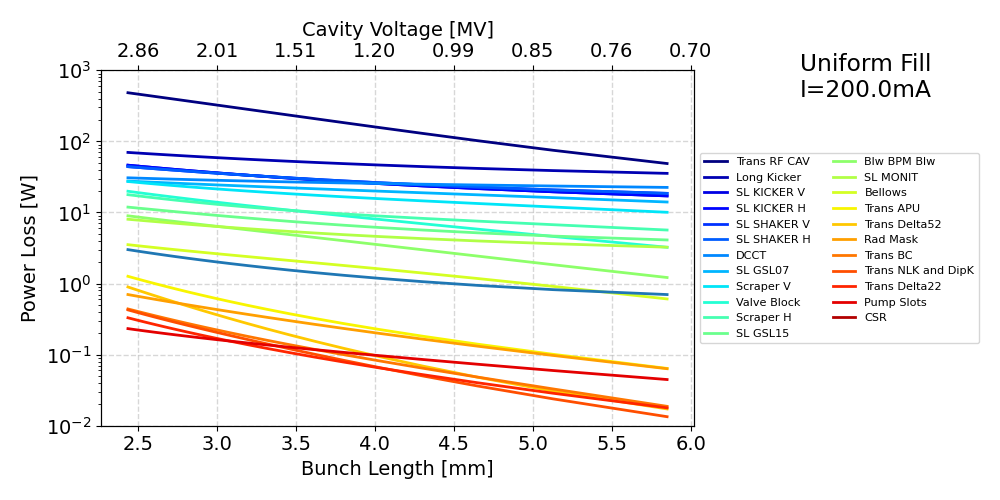
\includegraphics[width=0.48\textwidth]{vary_vgap_uniform_fill_curr200p00mA.png}
    \caption{Power loss for each component of the impedance budget model as function of the cavity voltage and bunch length.}
    \label{fig:model_vary_vgap}
\end{figure}
Figure~\ref{fig:model_vary_fillp} shows the model prediction for power loss for different filling patterns. Since most of the components are dominated by broad band impedances, the power loss do not depend too much on the filling pattern.
\begin{figure}
    \centering
    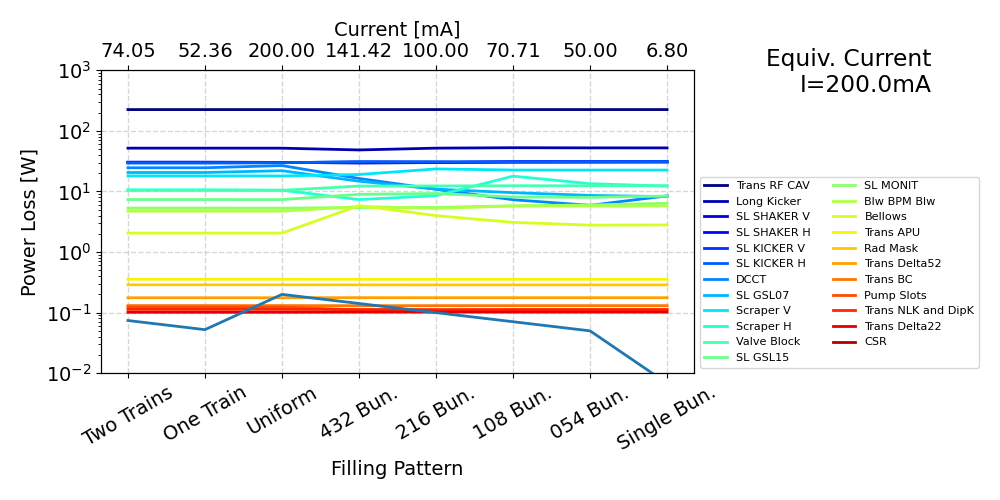
\includegraphics[width=0.48\textwidth]{vary_fillp_equivcurr200p00mA.png}
    \caption{Power loss for each component of the impedance budget model for several filling patterns. The total current used for each filling pattern was calculated using~\eqref{eq:power_broadband} so that the equivalent current in uniform filling was kept constant and equal to~\SI{200}{\milli\ampere}. The nomenclature~"$\!N$ Bun." refers to fillings with~$N$ equally spaced bunches.}
    \label{fig:model_vary_fillp}
\end{figure}

From these results we see that the taper transition of the superconducting rf cavities is the single component with the larger power loss reaching approximately~\SI{500}{\watt} at~\SI{200}{\milli\ampere} in uniform filling and~\SI{3}{\mega\volt} in the rf cavities. The second class of components with large power deposition are the striplines, ranging from~\SIrange{30}{90}{\watt} of deposited power.

\section{First Machine Shift (2023/07/25)}

Several temperature and pressure PVs were monitored during this study via archiver viewer.

\begin{itemize}
    \item Before the machine study there was \SI{100}{\milli\ampere} stored in the ring with nominal operation conditions;
    \item From this point, we tried to decrease the gap voltage of the cavity and increase the current so that the total power consumption of the cavity stayed constant;
    \item It was difficult to keep the beam stable in the longitudinal plane, so the process was slow;
    \item When we were at~\SI{107.5}{\milli\ampere} there was a beam dump of an so far unknown cause;
    \item We tried again, but another beam dump happened when we were at~\SI{110}{\milli\ampere};
    \item Another beam dump, now at a current lower than~\SI{100}{\milli\ampere};
    \item Francisco Gabriel, found out the cause for the beam dumps was the temperature of a mirror in the CEDRO beamline. We couldn't identify this earlier because this interlock was not properly mapped in the logging system;
    \item There was an access to the tunnel to solve a problem with the mirror movement system. In this intervention, they also found a problem with a valve that controls the water flow of the mirror's cooling system;
    \item Lunch;
\end{itemize}

\subsection{Non-uniform Filing}
\begin{itemize}
    \item After lunch we decided to change plans and study the heating under non-uniform fillings;
    \item We started by injecting a multi-bunch train of the EGun on the storage ring without changing the bucket list, such that all stored current is located on a single train. The bucket list index used was the bucket~\num{260}.
    \item In our first try the beam was dumped due to a problem in the IMBUIA beamline. There was another access to the tunnel to solve a problem related to the mirrors. We believe these problems with CEDRO and IMBUIA were not related to our study;
    \item We estimated the bunch profile using the horizontal and vertical~\gls{bbb} and the filling patter oscilloscope. Figure~\ref{fig:2023-07-25_onetrain_fill} shows the estimated filling pattern;
    \begin{figure}
        \centering
        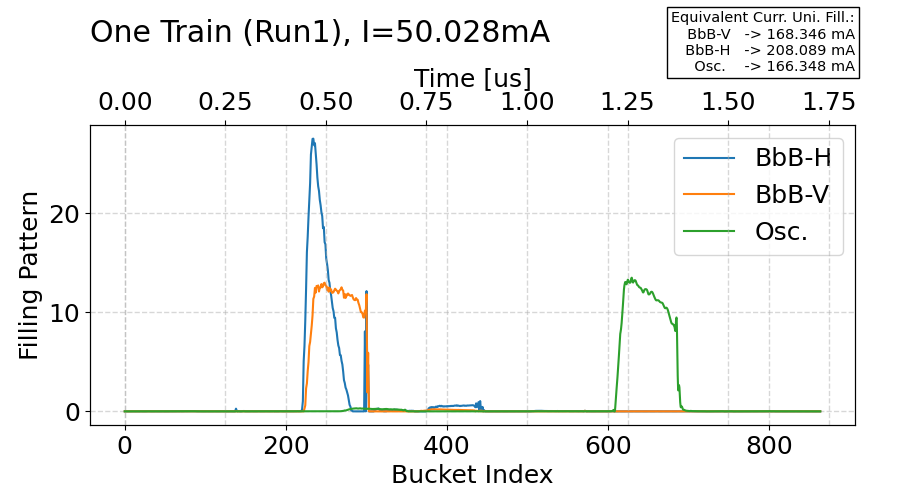
\includegraphics[width=0.48\textwidth]{2023-07-25_onetrain_run1_curr50p028mA.png}
        \caption{Filling pattern estimation by three different systems. Note the horizontal~\gls{bbb} gives a different filling, probably due to some non-optimal timing configuration. The text shows the equivalent current calculated using each filling.}
        \label{fig:2023-07-25_onetrain_fill}
    \end{figure}
    \item In the first try we reached~\SI{55}{\milli\ampere} and the beam was dumped due to interlock of the vacuum pump of sector 14M1. The valves from sector 13M2 and 14M1 were also closed;
    \item This same problem also happened for three more runs with the same filling pattern, now at smaller currents:~\SI{30}{\milli\ampere},~\SI{45}{\milli\ampere} and~\SI{39}{\milli\ampere}. We believe these problems are related to some narrow band impedance of the flange of the DCCT installed in sector 13C4. Such hypothesis is justified by the non-repeatability of the current at which these events happen and on the speed in which they occur. Analysing of the vacuum from that sector via archiver viewer, we noted several sudden pressure peaks, which is in contrast to the slow temperature and pressure rise of other sectors as seen in the graphs of Table~\ref{tab:graphics};
    \item To try to continue pushing up the estimated current for uniform filling without having these beam dumps, we injected a different filling pattern, with two trains. This filling pattern has a smaller number and intensity of revolution harmonics, and we hoped it would require a higher total stored current to dump the beam;
    \item With this filling pattern we reached~\SI{90}{\milli\ampere} of stored current, which amounts to~\SI{220}{\milli\ampere} in uniform fill in terms of broadband impedance induced heating. Figure~\ref{fig:2023-07-25_twotrain_fill} shows the estimated filling pattern and the currents in uniform filling.
    \begin{figure}
        \centering
        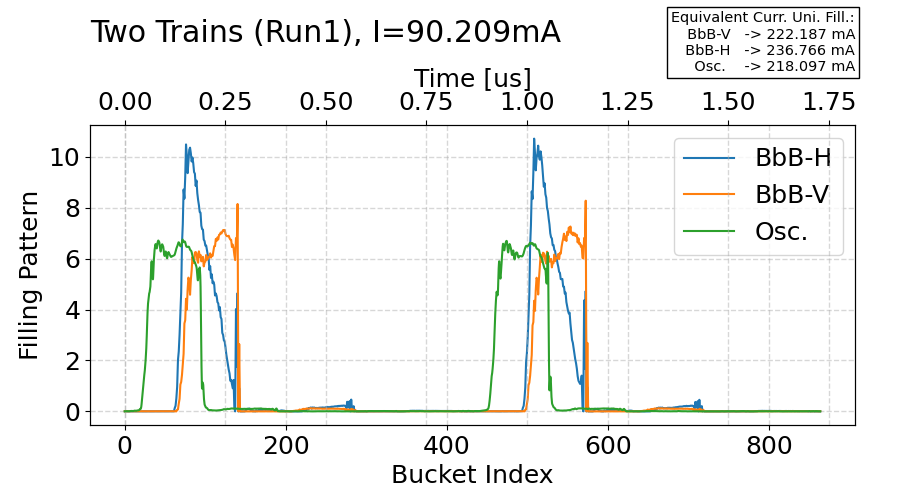
\includegraphics[width=0.48\textwidth]{2023-07-25_twotrains_run1_curr90p209mA.png}
        \caption{Filling pattern estimation by three different systems. Note the horizontal~\gls{bbb} gives a different filling, probably due to some non-optimal timing configuration. The text shows the equivalent current calculated using each filling.}
        \label{fig:2023-07-25_twotrain_fill}
    \end{figure}
    \item At this current the beam was dumped again due to the same interlock as before, when we were injecting in a single train. This sudden dump also corroborates with the hypothesis that relates it with narrow band impedances, because we reached currents whose equivalent uniform fill current are much larger than the ones we reached with the single train;
\end{itemize}

\subsection{Uniform Filling}
\begin{itemize}
    \item After this study we went back to trying to inject currents larger than~\SI{100}{\milli\ampere} in uniform filling with a lower voltage gap. This time we didn't care for the longitudinal stability, so the beam was always unstable;
    \item We started with a low gap voltage of~\SI{\approx1}{\mega\volt} and ramped up the current from zero. At~\SI{64}{\milli\ampere} the instability of the beam started to compromise the low level rf control and we had to increase the voltage;
    \item We followed this strategy along the rest of the experiment. We reached~\SI{150}{\milli\ampere} with a gap voltage of~\SI{1.5}{\mega\volt} and using~\SI{120}{\kilo\watt} of power;
    \item This \href{http://ais-eng-srv-ta.cnpem.br/archiver-viewer/index.html?pv=optimized_800(SI-Glob%3AAP-CurrInfo%3ACurrent-Mon)&pv=optimized_800(RA-TL%3ARF-Circulator-SIA%3APwrFwdOut-Mon)&pv=optimized_800(SI-02SB%3ARF-P7Cav%3AAmpVCav-Mon)&pv=optimized_800(SI-Glob%3ADI-BbBProc-L%3ASRAM_PEAK1)&from=2023-07-25T21%3A12%3A22.539Z&to=2023-07-25T22%3A12%3A22.539Z&ref=2023-07-25T00%3A03%3A59.368Z}{graphic} shows some variables related to the study described above.
\end{itemize}

\subsection{Final Remarks}

This first study indicates that the heating caused by the broad band impedance of the storage ring will not be an issue for operation with currents up to~\SI{200}{\milli\ampere}. We will perform more studies to confirm this assumption. In particular, we must make sure the beam dumps of this study were in fact being caused by narrow band impedances and fix the source of this contribution. We also need to let the beam stored for longer periods under the more demanding condition of filling pattern and total current so that the temperatures stabilize.

\section{Second Machine Shift (2023/08/01)}

In this second machine study we only pursued the idea related to more demanding filling patterns. We did not tried to increase the current beyond~\SI{100}{\milli\ampere}. Prior to this study, we accessed the tunnel and tightened the screws of the flange of the DCCT from sector 13C4. The screws allowed a modest tightening of approximately 1/3 of turns.

At around 8:00h the archiver crashed and the control netword became unstable. An intervention and restart of archiver was needed. All PVs took too long to connect to archiver, and the system only re-established all connections after lunch (around 13:00h). For this reason the first current ramp made in the morning is not archived. In this run, we reached~\SI{65}{\milli\ampere} with a single train in the machine. When we were ramping up to~\SI{70}{\milli\ampere} there was a beam dump to overheating of the vacuum window between the cavity and the waveguide. This interlock setpoint is~\SI{100}{\celsius} and could not be relaxed during the experiment. This temperature is highly influenced by the stability of the beam. Coupled-bunch oscillations generate extra power deposition on the region of the window. As an example, at nominal operation of~\SI{100}{\milli\ampere} at uniform filling with stable beam, the temperature only reaches~\SI{\approx52}{\celsius}.

During this first experiment we also fixed the timing configuration of the horizontal~\gls{bbb} so that its filling pattern estimate was in good agreement with the one from the vertical~\gls{bbb} and the oscilloscope. We had to change the phase of the front-end to accomplish this improvement in amplitude detection.

We went to lunch to wait for the Archiver to connect with all relevant PVs, including the one from the window. After lunch we inject a small current (\SI{35}{\milli\ampere}) in uniform filling to find the right phase for the horizontal~\gls{bbb} feedback coefficients. After that we went back to the single train filling. This time we also reached~\SI{65}{\milli\ampere} but did not go any further because of the temperature of the window. The \href{http://ais-eng-srv-ta.cnpem.br/archiver-viewer/?pv=optimized_800(SI-02SB%3ARF-P7Cav%3AGlassWinT-Mon)&pv=optimized_800(SI-Glob%3AAP-CurrInfo%3ACurrent-Mon)&from=2023-08-01T13%3A04%3A34.194Z&to=2023-08-01T21%3A04%3A34.194Z&ref=2023-08-03T19%3A20%3A55.734Z}{graph} shows the temperature of the window and the stored current during this experiment. Figure~\ref{fig:2023-08-01_onetrain_fill}
\begin{figure}
    \centering
    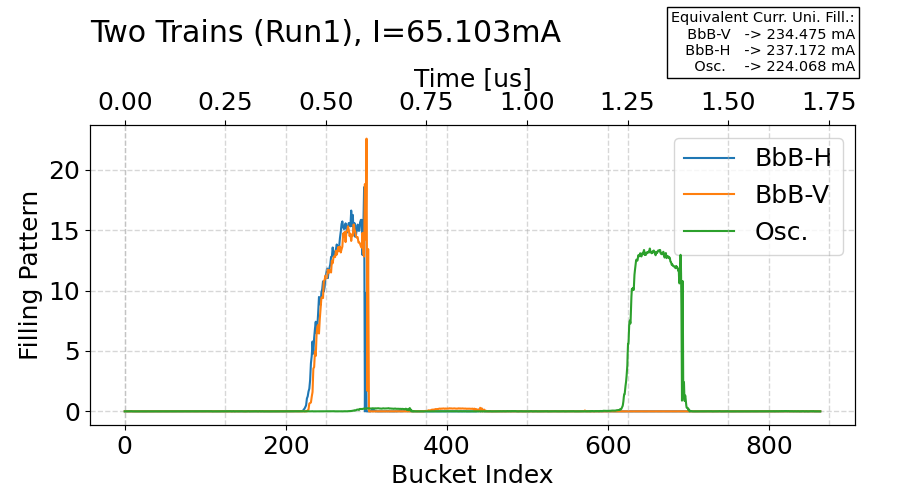
\includegraphics[width=0.48\textwidth]{2023-08-01_trains1_run3_curr65p103.png}
    \caption{Filling pattern estimation by three different systems. The text shows the equivalent current calculated using each filling.}
    \label{fig:2023-08-01_onetrain_fill}
\end{figure}
shows the equivalent current reached in this situation. We kept the beam with this current in top-up mode for some time to analyse the evolution of the pressure and temperature of the components. We didn't notice any problems related to the pressure, but some measurements of temperature from sector~\num{1} increased significantly and did not stabilize during the whole experiment, reaching~\SI{\approx53}{\celsius} before we dumped the beam. We don't know yet to which component this measurement refers, but we will access the tunnel next Monday morning (2023/08/06) to map the sensor position. Most probably though, it refers to the vertical scraper.

Next, we injected the beam in two trains. In this configuration we could reach~\SI{90}{\milli\ampere} and the temperature of the window was kept at~\SI{96}{\celsius}. The same heating problem was observed in sector 1. Figure~\ref{fig:2023-08-01_twotrains_fill}
\begin{figure}
    \centering
    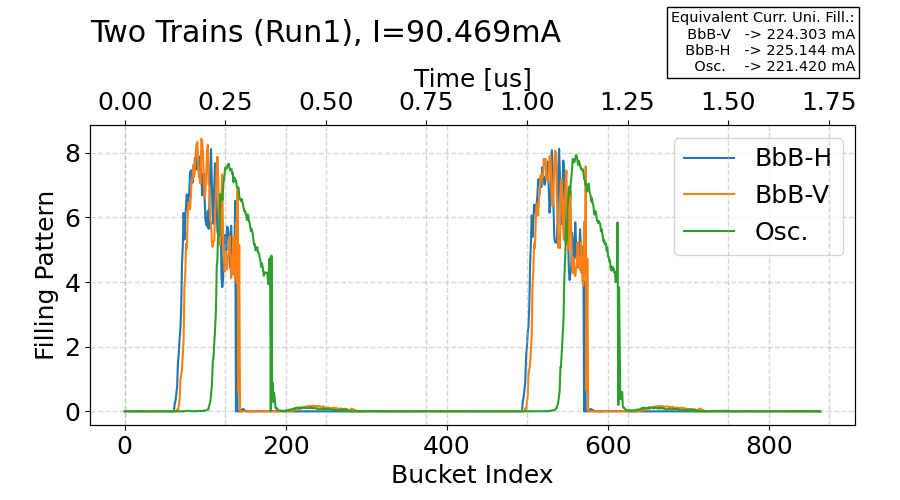
\includegraphics[width=0.48\textwidth]{2023-08-01_trains2_run1_curr90p469.png}
    \caption{Filling pattern estimation by three different systems. The text shows the equivalent current calculated using each filling.}
    \label{fig:2023-08-01_twotrains_fill}
\end{figure}
shows the equivalent current of this filling. The similarity to the single train estimated current together with the same heating behavior, corroborates with the hypothesis of broadband induced power on the component close to the sensor.

We ended the machine shift at around 17:00h to start recovering the machine for users operation.

\section{Conclusion}
The mode 1 instability induced by HCs in electron storage rings was investigated. The instability was reproduced with 1 macroparticle per bunch in tracking simulations and accurately predicted with a linear theory for Gaussian bunches slightly adapted to a HC system. Determining the most appropriate measure of average incoherent frequency remains an open question. Instability occurs when two radial modes approach zero frequency. A direct conclusion is that parameters that either increase the incoherent synchrotron frequency or decrease the negative coherent shifts of coupled-bunch mode 1 are beneficial to increase the current or HC voltage threshold. In 4\textsuperscript{th} generation synchrotrons, the ultralow emittances requires reduced momentum compaction factor and sychrotron frequency, which make new machines with HCs more susceptible to the mode 1 instability.


\section{Acknowledgments}
The authors thank Liu Lin and Ximenes Resende for fruitful discussions and suggestions.
%
% only for "biblatex"
%
\ifboolexpr{bool{jacowbiblatex}}%
	{\printbibliography}%
	{%
	% "biblatex" is not used, go the "manual" way
	
	%\begin{thebibliography}{99}   % Use for  10-99  references
	\begin{thebibliography}{9} % Use for 1-9 references

   \bibitem{Lima:IPAC22-TUPOST014}
   A. P. B. Lima, I. Carvalho de Almeida, D. Daminelli, R. H. A. Farias, M. Hoffmann Wallner, and F. K. G. Hoshino,
   \textquotedblleft{Sirius Storage Ring RF System Status Update}\textquotedblright,
   in \emph{Proc. IPAC’22}, Bangkok, Thailand, Jun. 2022, pp. 872--875.
   \url{doi:10.18429/JACoW-IPAC2022-TUPOST014}

    \bibitem{Venturini2018}
    M. Venturini,
    ``Passive higher-harmonic rf cavities with general settings and multibunch instabilities in electron storage rings,''
    \emph{Phys. Rev. Accel. Beams 21} 114404 (2018)

    \bibitem{He2022b}
    T. He,
    \textquotedblleft Novel perturbation method for judging the stability of the equilibrium solution in the presence of passive harmonic cavities \textquotedblright in
    \emph{Phys. Rev. Accel. Beams} \textbf{25}, 094402 (2022)

    \bibitem{He2022a}
    T. He, W. Li, Z. Bai, and L. Wang,
    \textquotedblleft Periodic transient beam loading effect with passive harmonic cavities in electron storage rings\textquotedblright~in \emph{Phys. Rev. Accel. Beams} \textbf{25}, 024401 (2022)
    
    \bibitem{Cullinan2024}
    F. J. Cullinan, \AA{}. Andersson, J. Breunlin, M. Brosi, and P. F. Tavares,
    \textquotedblleft Experimental observation of a mode-1 instability driven by Landau cavities in a storage ring \textquotedblright in \emph{Phys. Rev. Accel. Beams 27}, 044403 (2024)

    \bibitem{CollectiveEffectsRepo}
    F. H. de Sá and M. B. Alves,
    ``pycolleff and cppcolleff: Modules for impedance analysis and wake-field induced instabilities evaluation'' (2023),
    \url{https://doi.org/10.5281/zenodo.8088076}

    \bibitem{Suzuki1983}
    T.~Suzuki, Y.~Chin, and K.~Satoh,
    \textquotedblleft Mode Coupling Theory and Bunch Lengthening in {SPEAR} {II} \textquotedblright
    \emph{Part. Accel.} \textbf{13} (1983), 179-198,
    KEK Preprint 82-26

    \bibitem{AlvesSa2023}
    M. B. Alves and F. H. de S\'a,
    ``Equilibrium of longitudinal bunch distributions in electron storage rings with arbitrary impedance sources and generic filling patterns,''
    \emph{Phys. Rev. Accel. Beams 26}, 094402 (2023)

    \bibitem{Lindberg2018}
    R. R. Lindberg,
    ``Theory of coupled-bunch longitudinal instabilities in a storage ring for arbitrary rf potentials,''
    \emph{Phys. Rev. Accel. Beams 21}, 124402 (2018)
	\end{thebibliography}
} % end \ifboolexpr


\end{document}

